\documentclass{subfiles}

\begin{document}

\section{Introduction}


\subsection{The Importance of Dead Wood}

\par The value of dead trees from a biodiversity management perspective is large. Once a tree dies, its contribution to our ecosystem continues. The woody structure remains for centuries and it contributes to forest regeneration while providing resources for numerous surrounding organisms \cite{Franklin1987}. As an indication, more than 4000 species inhabit dead wood in Finland \cite{Siitonen2001}, where an estimate of 1000 species has been extinct \cite{Hanski2000}. These species do not only include animals and birds but also organisms, like fungi. Fungi contributes to wood decaying, formation of hollows and biodiversity, which is an important factor for a resilient ecosystem \cite{Peterson2000}. Observing the changes of fungal diversity on decaying wood has an increased interest in science  \cite{Abrego2011} \cite{Stokland2011} \cite{Lonsdale2008} in order to ensure the continuous existence of decaying wood in forests. 




\par In Australia, tree hollows play a significant role in managing biodiversity. Nearly all arboreal mammals rely on hollows with the exception of the Koala and perhaps Ringtail Possums that preferentially make a stick nest, but they use hollows as well. Additionally, a large number of Australian bird species rely on hollows for shelters \cite{Gibbons2002}. Nevertheless, Australia has no real hollow creators unlike the northern hemisphere (e.g. Woodpeckers), and therefore it relies predominantly on natural processes of limb breakage, insect and fungal attack when access points are provided through damage caused by wind, storms and fire. 

\par This kind of hollows take hundreds of years to form and because of that it is more likely to exist on dead trees. In Australia, studies predict shortage of hollows for colonisation in the near future \cite{Lindenmayer2010} \cite{Goldingay2009}. Therefore automated detection of them plays a significant role in protecting those animals. As an indicator of the importance of hollows in managing biodiversity, a list of a few of the species that rely on hollows was provided by the Forestry Corporation of NSW. Those species are shown at Figure \ref{fig:Birds}. According to the Department of the Environment of Australian Government and the Government of Western Australia, six of them are  protected, threatened or close to extinct \cite{AustraliaExtinct1999}  \cite{AustraliaExtince2015}. Figure \ref{fig:Birds} shows the species from the provided list and the six protected species have a red border and their names are bold in the description. 

\par For the aforementioned reasons, monitoring dead trees is essential for having a resilient ecosystem. Nevertheless, the distribution of dead trees significantly varies making detection of them difficult \cite{Kim2009}. Remote sensing approaches has been introduce to automate the process of monitoring forest and further increase the spatial resolution of the monitored area. The following section gives an overview of the related work undertaken in Remote Sensing. 



\afterpage{
	\begin{figure} 
		\centering
		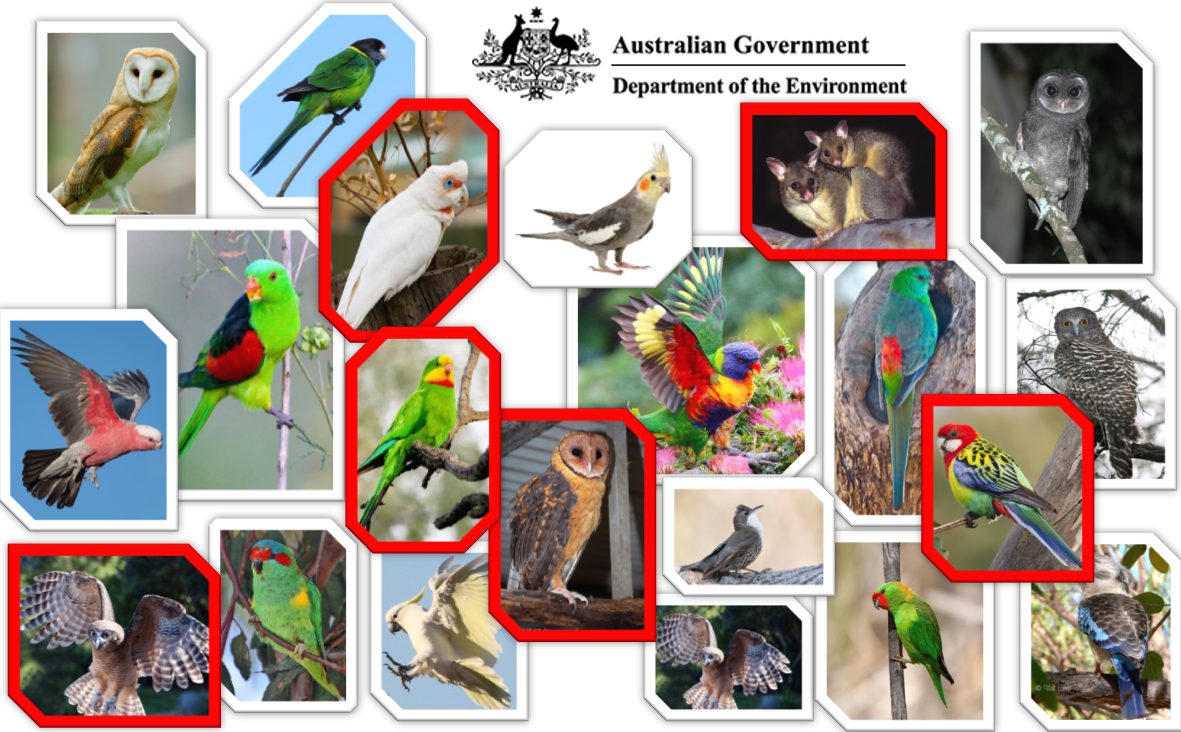
\includegraphics[width=\textwidth]{img/dead/Birds}
		\caption[Animals Closes to Exctinction]{A number of species that rely on tree hollows of which the red ones / bold ones are close to extinction: Kookaburra, Sulphur Crested Cockatoo, \textbf{Corella},  Crimson Rosella, Eastern Rosella,  Galah, Rainbow Lorikeet,  Musk Lorikeet, Little Lorikeet , Red-winged Parrot,  \textbf{Superb Parrot}, Cockatiel,   Australian Ringneck (Parrot),  Red-rumped Parrot,   Powerful Owl,    Sooty Ow,        Barking Owl, \textbf{Masked Owl},  \textbf{Barn Owl},  White-throated Treecreeper, Hollow Owl, \textbf{Brush-tailed Possum} (mammal) \footnotemark}
		\label{fig:Birds}
	\end{figure}
	\footnotetext{    	
		The images of the birds were taken from the following links (Retrieved on the 27th of April 2016):  
		Kookaburra: \url{<http://tenrandomfacts.com/blue-winged-kookaburra/>}, 
		Sulphur Crested Cockatoo: \url{<http://aussiegal7.deviantart.com/art/Sulphur-Crested-Cockatoo-08-153341893>},
		Corella: \url{<http://www.theparrotplace.co.nz/all-about-parrots/long-billed-corella/},     	Superb Parrot: \url{<http://www.davidkphotography.com/?showimage=637>},
		Crimson Rosella: \url{<http://25.media.tumblr.com/tumblr_m3mo89c40r1r4t9h1o1_1280.jpg>},
		Eastern Rosella: \url{<http://2.bp.blogspot.com/-pYxw51WjSOY/UB-LEFgd2KI/AAAAAAAAAWg/9z60PUWE6TE/s1600/_GJS6601-as-Smart-Object-1.jpg>},
		Rainbow Lorikeet: \url{<https://www.reddit.com/r/pics/comments/328fvc/a_rainbow_lorikeet_found_in_coastal_regions/>},     	Musk Lorikeet: \url{<http://www.rymich.com/girraween/photos/animals/birds/medium/glossopsitta_concinna/glossopsitta_concinna_001.jpg>},     	Little Lorikeet: \url{<http://www.pbase.com/sjmurray/psittacidae>},     	Red-winged Parrot: \url{<https://www.pinterest.com/pin/395894623469889727/>}, Cockatiel: \url{<http://up.parsipet.ir/uploads/Cockatiels-for-sale.jpg>},     	Australian Ringneck (Parrot): \url{<http://ontheroadmagazine.com.au/wp-content/uploads/2015/09/Twenty-eight-parrot-2-min.jpg>},     	Red-rumped Parrot: \url{<http://parrotfacts.net/wp-content/uploads/Red-Rumped-Parrot-on-a-tree.jpg>},     	Powerful Owl: \url{<http://farm1.staticflickr.com/219/495796536_f78dac04c1.jpg>},     	Sooty Owl: \url{<ttp://www.mariewinn.com/marieblog/uploaded_images/screech2-738532.jpg},     	Barking Owl: \url{<http://www.pcpimages.com/Nature-and-Wildlife/Birds/i-7JKSTp5/1/L/owl\%20\%281\%20of\%201\%29-L.jpg>},     	Masked Owl: \url{<http://www.survival.org.au/images/birds/masked_owl_2_600.jpg>},  	Galah: \url{https://www.pinterest.com/pin/537546905498955709/>},   	White-throated Treecreeper: \url{<https://geoffpark.files.wordpress.com/2011/09/female-white-throated-treecreeper.jpg>}, Hollow Owl: \url{<http://www.mariewinn.com/marieblog/uploaded_images/screech2-738532.jpg>} }
}





\subsection{Related Work}

\par Remote Sensing was introduced for automatically detecting dead trees, because fieldwork is time consuming considering their variance spread and the size of the relevant forests. From a classification perceptive, the task of identifying dead standing and dead fallen trees is different. Fallen trees are identified by detecting segments or line-like features on the terrain surface using LiDAR data \cite{Polewski2015} \cite{Mucke2013}. Regarding standing dead trees, their shape (reduced number of leaves or broken branches) \cite{Yao2012} and light reflectance (less green light illuminated) \cite{Pasher2009} are important factors for identifying them.


\par Previous work on dead standing trees detection performs single tree crown delineation before health assessment \cite{Yao2012} \cite{Shendryk2016_DeadTrees}. Tree-crown delineation is usually done by detecting local maxima from the canopy height model (CHM) and then segmenting trees with watershed algorithm \cite{Popescu2003}. Improvements has been achieved by introducing markers controlled watershed \cite{Jing2012} and structural elements of tree crowns with different sizes \cite{Hu2014}. Additionally, Popescu and Zhao analyse the vertical distribution of the LiDAR points in conjunction with the local maximum filtering of CHM \cite{Popescu2008}.


\par  In the case of Eucalyptus, single tree detection is a challenge on its own, due to their irregular structure and multiple trunk splits. In other words, each tree trunks splits create a local maximum leading into over-segmentation when tree crowns are detected by local maxima filtering. Shendryk published a eucalyptus delineation algorithm that starts segmentation from bottom to top. In this paper, the trunks point cloud is separated from the leaves and individual trunks are identified before proceeding to crown segmentation \cite{Shendryk2016_treeDeliniation}. Nevertheless, for that project only 17 flightlines of LiDAR data were collected. The density resolution starts from 12 points/$m^2$ and goes up to 36 points/$m^2$ around forested areas. For small research projects capturing this high resolution is acceptable, but for commercial use and larger areas, the density of data collected is above the optimal resolution for a cost effective versus quality acquisition \cite{Lovell2005}. The project of this thesis is much larger. The resolution of our acquired LiDAR data has an average of four pulses per square meter,{\color{blue} which is considered an optimal resolution in relation to the cost}. But because of the tree height (up to $43m$ according to the fieldwork), a small amount of pulse intensity reached the trunks and the recordered waveform do not include enough information for individual trunk detection.  An example of this project's discrete LiDAR data is shown in Figure \ref{fig:NoTrunks} and the missing information about the trunks is depicted.

\begin{figure} [h!]
	\centering
	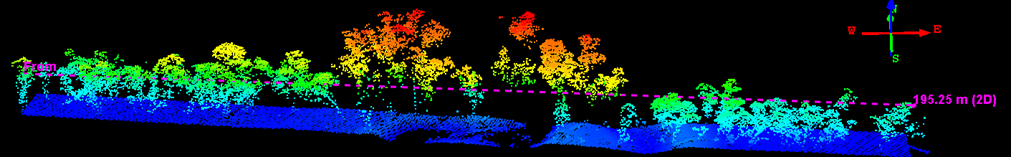
\includegraphics[trim={7cm 0 1.7cm 0},clip,width=\textwidth]{img/dead/TreesNoTrunks}
	\caption{LiDAR point cloud showing that there are very limited points reflected from tree trunks.}
	\label{fig:NoTrunks}
\end{figure}


{\color{red} ***Note read again to make sure it matches OK}
\par The acquired data are full-waveform LiDAR data. Traditional ways of interpreting FW LiDAR data, suggests extraction of a denser points cloud using Gaussian decomposition ~\cite{Neuenschwander2009} ~\cite{Reitberger2008}. Nevertheless, in this project we uses the open source software DASOS. DASOS was influenced by Persson et al ~\cite{Persson2005}, who used voxelisation to visualise the waveforms . But, it does not only uses voxelisation for visualisations but also for extracting metrics useful in classification. It further normalises the intensities so that equal pulse length exists inside each voxel, making intensities more meaningful. It is further seems that the literature is moving towards voxelisation with promising results obtained at recent publication on tree species classification ~\cite{Cao2016}. 

Here, it is introduced an approach for quick dead tree detection derived from the boost cascade approach ~\cite{Viola2001} but extended into 3D. This approach further contains similarities of the 3D tree shape signatures proposed by Dong, 2009, for distinguishing Oaks from Douglas fir tree crowns ~\cite{Dong2009}. 





%\subsection{Potentially add Objectives???}







\section{Materials}

\subsection{Study Area} \label{sec:StudyArea}

The study area (Figure \ref{fig:StudyArea}) is a native River Red Gum (Eucalyptus camaldulensis) forest  of size $542km^2$ in south-eastern Australia. The regeneration of the eucalyptus is extremely dependant in floods and therefore, their distribution in respect to density, health and age is highly variance \cite{Kerle2005}. Additionally, the height of Eucalyptus camaldulensis reaches up to $30-40m$ and their structural complexity is high with multiple trunk splits \cite{Wilson1995}. The size and structure of the forest, with a human as reference, is depicted in Figure \ref{fig:EucalyptusSize}, while examples of the variance shape of dead trees is shown in Figure~\ref{fig:DeadTreesExamplePhotos}. 

\begin{figure} [h!]
	\centering
	\begin{framed}
		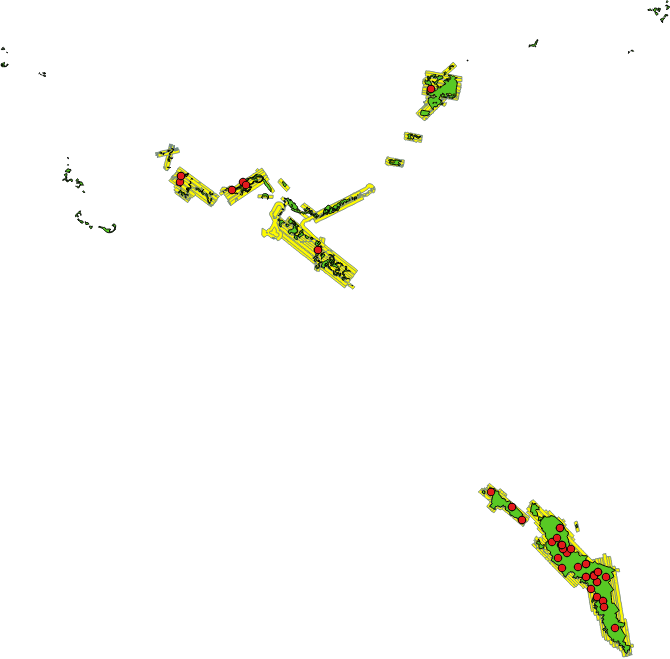
\includegraphics[width=0.965\textwidth]{img/dead/StudyArea}
	\end{framed}
	\caption{The study area is depicted by green ($542km^2$), the yellow strips are the LiDAR flightlines and the red dots are the position of the field plots.{\color{red}**Note: this image many need to be removed due to confidentiality of the company. I will talk with them and hopefully it will be ok.}}
	\label{fig:StudyArea}
\end{figure}

\begin{figure} [h!]
	\centering
	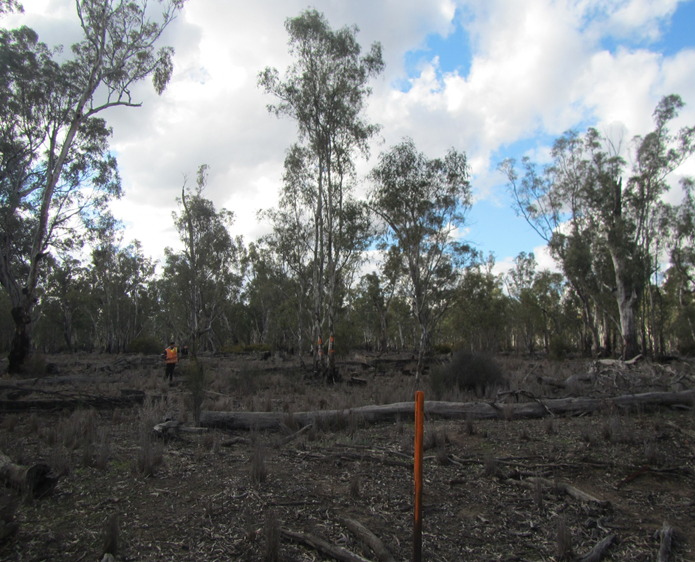
\includegraphics[width=0.965\textwidth]{img/dead/Eucalyptus.png}
	\caption{Structure of Red Gum Forest in south-eastern Australia.}
	\label{fig:EucalyptusSize}
\end{figure}

\begin{figure} [h!]
	\centering
	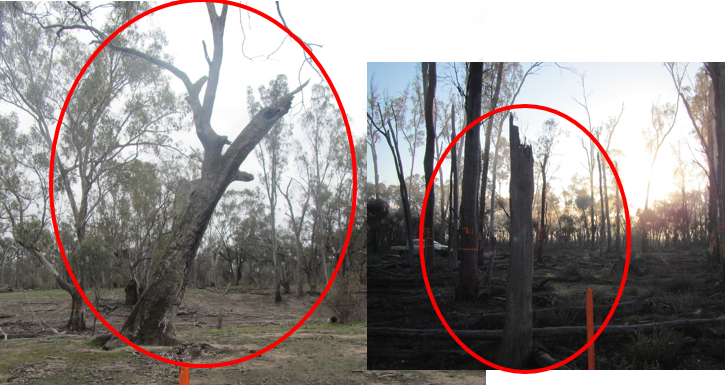
\includegraphics[width=0.965\textwidth]{img/dead/DeadTreesExamplePhotos}
	\caption{Example of dead trees indicating their variance in shape.}
	\label{fig:DeadTreesExamplePhotos}
\end{figure}

\subsection{Acquired full-waveform LiDAR data}\label{sec:AcquiredData}

\par Multiple-echo, full-waveform (FW) LiDAR data are supplied by RPS Australia East Pty Ltd. The data were acquired from 900m above ground level, using the Trimble AX60 Airborne LiDAR sensor, which was released in October 2013 \cite{Trimble}. The wavelength of the emitted laser was 1062nm, the maximum scan angle was 60 degrees, and the pulse rate was 400kHz. The acquisition was held from the 6th of March till the 31st of March 2015.  The collected LiDAR were delivered into 206 flightlines, of which 13 are cross runs used for geometric correction. There is also a 30\% of swath overlap. The point spacing along and across the track  is 0.48m and the average point spacing is 4.3 points per square meter. Figure \ref{fig:DeadTreeInLiDAR} shows an example of a dead tree in respect to the acquired discrete LiDAR point cloud.   Detailed information about FW LiDAR related concepts are given in section \ref{AcquireData}.



\begin{figure} [h!]
	\centering
	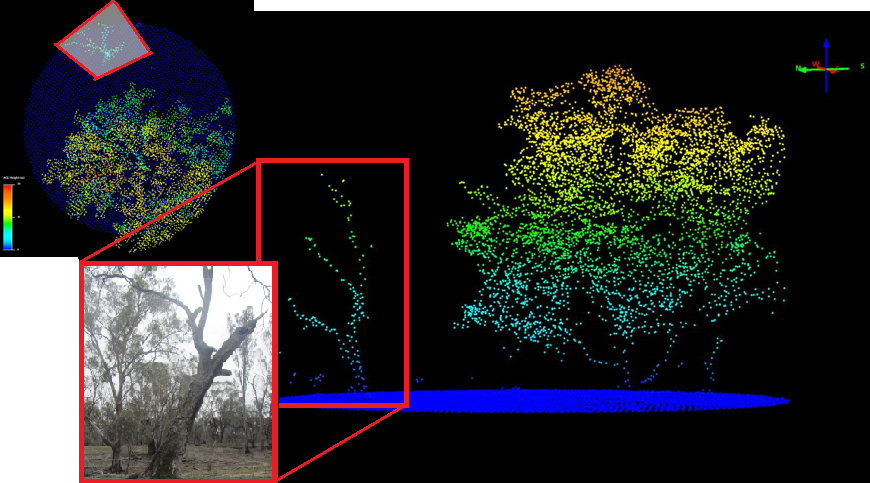
\includegraphics[width=\textwidth]{img/dead/DeadTreeInLiDAR}
	\caption{Example of a dead tree in relation to the discrete LiDAR point cloud.}
	\label{fig:DeadTreeInLiDAR}
\end{figure}



\subsection{Field Data}\label{sec:fieldData}

\par The field data were collected in July 2015 during the winter season of Australia and they include tree and canopy related measurements on circular plots. There are 33 plots with radius 35.68m and area 0.4ha  allocated randomly inside the study area. On these plots, a total of 2386 trees were individually measured.  Tree measurements include the geo-location, the trunk diameter at the standard height of 1.3m (breast heigh), height, species and health conditions (i.e. dead or alive). The geo-location of each tree is defined by the magnetic bearing from the centroid of the plot in degrees (range $[1,360]$) and the distance from the centroid in meters. The northing and easting coordinates of the geo-location of each tree were calculated in post-processing. Here is worth mentioning that a single tree may be recorded as multiple trees if there is a trunk split bellow the breast height of 1.3m. Furthermore, 91.59\% are River Red Gum and the rest are Black Box (Eucalyptus largiflorens) and Wattle group (Acacia spp.). 

\par Inside the field data, there are 260 dead trees recorded. Nevertheless, not all of those trees are considered useful for biodiversity. Dead trees with big Diameter at Breast Height (DBH) are more likely to contain hollows. Additionally, trees with DBH smaller than the footprint spacing of the LiDAR data are not identifiable from the FW LiDAR data. Table \ref{tab:DBH} shows the number of dead and alive trees in respect to their DBH. 

\begin{table}[!h]
	\centering
	\begin{tabular}{| l || c | c | }
		\hline		
		\textbf{DBH (cm)} &\textbf{Dead Trees} & \textbf{Alive Trees }\\	
		\hline			
		\hline			
		\textbf{>2000} & 0 & 1\\
		\hline			
		\textbf{1000-2000} & 7 & 21\\
		\hline			
		\textbf{600-1000} & 8 & 146\\
		\hline			
		\textbf{400-600} & 26 & 290\\
		\hline			
		\textbf{300-400} & 32 & 286\\
		\hline			
		\textbf{200-300} & 50 & 462\\
		\hline			
		\textbf{100-200} &125 & 904\\
		\hline			
		\textbf{<100} & 11 & 16\\
		\hline			
		\textbf{Total} & 260 & 2126 \\
		\hline  
	\end{tabular}
	\caption{Number of trees according to their DBH}
\end{table}

\par Please note that the aforementioned field data were provided by Forestry Corporation of NSW, Wauchope, Australia and Interpine Ltd Group, New Zealand. For this thesis, a case study for collecting field data was conducted in New Forest, UK. This helped to better understand classification challenges in forestry applications. More information about this study is provided in Appendix \ref{Fieldwork}.



\section{Classification Challenges}\label{sec:ClassficationChallenges}
\par This section focuses on the challenges faced while working on the detection of dead standing eucalyptuses. Table \ref{tab:ClassificationChallenges} underlines these challenges, categorised into three groups: the nature of the study area, the acquired data and the field data. All these challenges influence the quality of the classifier and the accuracy of the results. 


\begin{table}[!h]
	\centering
	\begin{tabular}{| p{0.3\linewidth} ||  p{0.3\linewidth} ||  p{0.3\linewidth} | }
		\hline		
		\textbf{Study Area} &\textbf{Acquired Data} & \textbf{Field Data}\\	
		\hline			
		\hline
		\tabitem 	The study area is a native eucalyptus forest. Native forests contain trees of different ages and heights. The height of a dead tree could be within the range of [1.5,40] meters.\newline
		\tabitem There is a high variance in the density of the forest. Sometimes the testing/training priors of the small dead trees may contain information from either nearby alive trees or ground.  \newline 
		\tabitem A tree may have dead branches but still be alive. \newline
		\tabitem Eucalyptus trees have irregular shapes and multiple trunk splits making tree delineation to require very dense acquired data. 
		 &
		  \tabitem The pulse density of the acquired data does not allow bottom to top tree delineation. Crown detection from DEM (top) leads to over-segmentation due to the multiple trunk-splits. We, therefore, investigate the performance of object detection algorithms that do not require tree delineation.\newline
		  \tabitem An important factor of identifying dead trees is the light reflectance, but for this project this kind of data (i.e. coloured imagery) was not acquired. Therefore, the classifier is only trained on tree shapes. But the shape of the tree is not an independent factor of identifying dead trees, since a tree may not have leaves but still be alive.				 
		 & 
         \tabitem If a tree has a trunk split below the 1.3m height, then it is recorded as multiple trees within the field data. This results into an inconsistency of the "one tree" concept.  \newline
		 \tabitem They contain small trees, which are non detectable from the acquired data. \newline
		 \tabitem The accuracy of the geo-spatial positions is unknown. Even though it is claimed to be within centimetres, there are trees clearing appearing on the ground, once visualised on top of the DEM. An example:
		  \raisebox{-\totalheight}{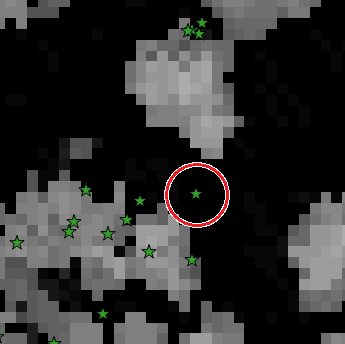
\includegraphics[width=0.3\textwidth]{img/dead/TreeOnGround}}
		 \\
	
		\hline  
	\end{tabular}
	\caption{The Classification challenges of automated detection of dead eucalyptuses}
	\label{tab:ClassificationChallenges}
\end{table}

\section{Methods and Algorithms}

\par This section provides an explanation of the algorithms implemented. An overview of the work flow is given here: 
\begin{enumerate}
	\item Subtraction of the Digital Terrain Model (DTM) from the FW LiDAR data
	\item {\color{blue} Generation of training feature vectors characterising dead and alive trees, as well as testing samples of unknown population
	\item Identification of the most important relevant features using random forest}
	\item Generation of a probabilistic field using a weighted k-nearest neighbour (KNN) algorithm. 
	\item Filtering 
	\item Height histogram and ground pixels removal
	\item Thresholding dead pixels from alive, filtering, applying a seed growth algorithm for grouping nearby pixels and assignment of dead trees position.  
\end{enumerate}

\subsection{Subtract DTM from FW LiDAR}\label{sec:DTMsub}

\par A feature was implemented in DASOS for subracting pre-calculated Digital Terrain Model (DTM) saved into .bil files. Generating a DTM is beyond the scope of this research and the DTM files used were provided by Interpine Ltd Group. The provided DTM files were generated using the Quick Terrain Modeller from discrete LiDAR using the parameters shown in Figure \ref{fig:DTM_parameters}.

\begin{figure} [h!]
	\centering
	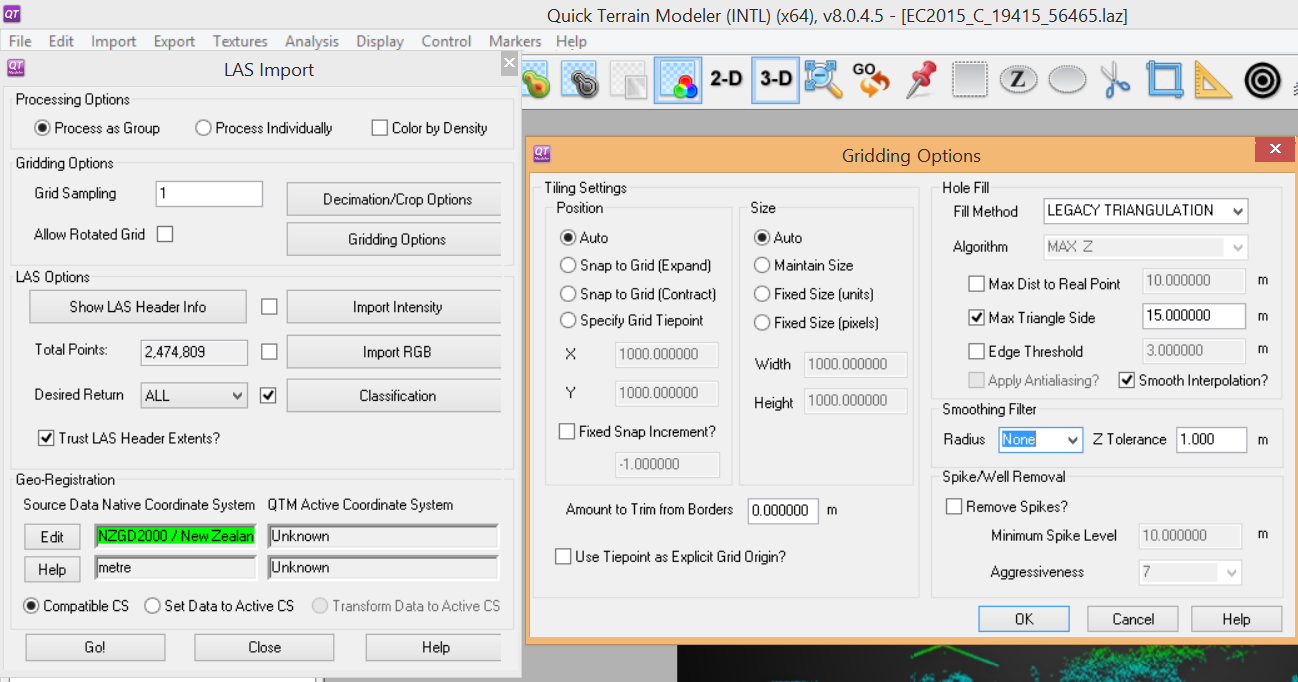
\includegraphics[width=\textwidth]{img/dead/DTM_parameters}
	\caption{Parameters used in Quick Terrain Modeller to obtain the DTM used here.}
	\label{fig:DTM_parameters}
\end{figure}


\par The subtraction of the DTM is done during the voxelisation (Section \ref{DASOS_Voxelisation}). The terrain height is subtracted from the position of the sample before it is inserted into the volume. Please note that each terrain value is not subtracted from the origin of its pulse but from the position of each sample since the terrain value at the origin and the terrain value at the position of a sample may differ. 
\par Figure \ref{fig:height_minus_dtm} shows an example of a DEM generated before and after the subtraction using DASOS. 


\begin{figure} [h!]			
	\begin{subfigure}[t]{.49\textwidth}
		
		\centering
		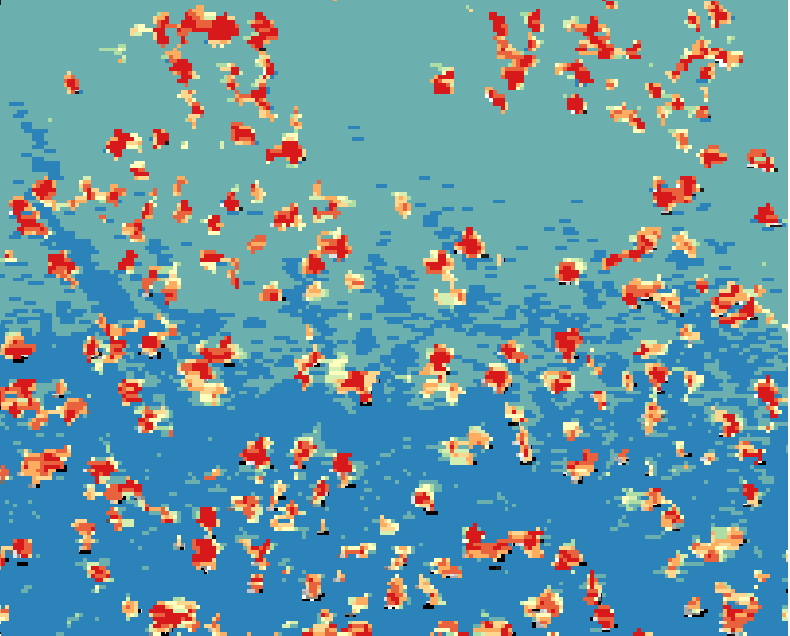
\includegraphics[width=\textwidth]{img/dead/height}
		\caption{The DEM before subtracting the DTM}
		\label{fig:height}
	\end{subfigure} \hfill
	\begin{subfigure}[t]{.49\textwidth}
		\centering
		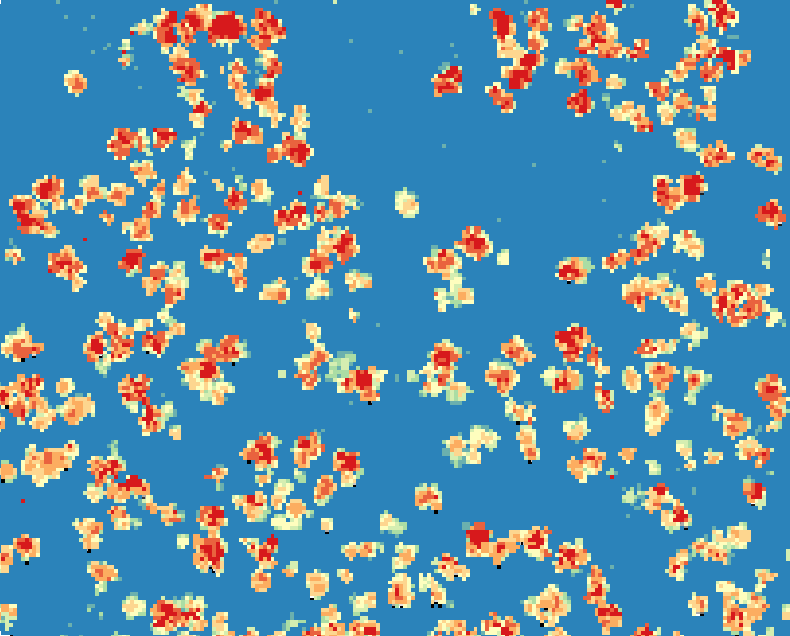
\includegraphics[width=\textwidth]{img/dead/height_dtm}
		\caption{The DEM after subtracting the DTM} 
		\label{fig:height_dtm}
	\end{subfigure} \hfill
	\caption[Before and after subtracting the DTM.]{The difference of the DEM before and after subtracting the terrain height. The  red indicates big height, while the darker the blue is the lower the DEM is.}  
	\label{fig:height_minus_dtm} 
\end{figure}


\subsection{Generating feature vectors using DASOS}\label{sec:3DpriorsGeneration}

\par The feature vectors is a new feature of DASOS (version 2), which was released on the 20th January 2017 \cite{DASOS_v2}. The dead tree detection is its first application. This feature is useful for characterising object inside the 3D space (e.g. trees). For each column of interest within the voxelised FW LiDAR data, information around its local area are exported as feature vector. Multiple feature vectors are listed within .csv files for easy manipulation into software packages specialised in statistical analysis like R and matlab. There are two types of exported information from these local areas: processed and raw. If the processed option is chosen, then information like the distribution of non-empty voxels and the standard deviation of heights are listed. A sample of the exported processed information along with explanations is given in Table \ref{tab:DASOSpriorsExplanationDead}, while the entire list is provided within the Appendix \ref{DASOS_userGuide}. If the exported parameters are raw, then the corresponding intensity values of the local area's voxels are exported. {\color{blue} Additionally, there are two available shapes of the local area from where the features are extracted (the cuboid and the cylinder). The size of shape is also user defined. Here, the aforementioned feature of DASOS is used for generating feature vectors used as a likelihood in the classifier. }


\begin{table}[!h]
	\centering
	\begin{tabular}{|p{0.85cm}|p{4.5cm}|p{7.8cm}|}
		\toprule
		\multicolumn{3}{|c|}{\textbf{Explanation of some features of DASOS's 3D priors that proved }}\\ 
		\multicolumn{3}{|c|}{\textbf{to be useful for building the classifier}} \\
		\midrule
		\textbf{No}&\textbf{Label} & \textbf{Description} \\ 
        \hline
		1&Height\_Middle\_Column& The height of the middle column of the prior
		\\
		\hline
		&Height\_Mean& The Mean height of all the columns included in the template\\
		\hline
		&Height\_Median& The Median height of all the columns included in the template
		\\
		\hline
		1 &Height\_Std&The Standard Deviation of the heights of the columns included in the template \\
		\hline
		2&Top\_Patch\_Len\_Std& The Standard Deviation of all the top patches \\
		\hline
		3&Dis\_Std& The Standard Deviation of the distances between the central voxel and every voxel that contains an intensity above the isolevel\\
		\hline
		4&Per\_Int\_Above\_Iso& Percentage of voxels that contain an intensity above the isolevel\\
		\hline
		5&Top\_Patch\_Len\_Mean& The Mean length of all the top patches\\
		\hline
		&Top\_Patch\_Len\_Median& The Median length of all the top patches \\
		\hline
		7&Dis\_Mean& Mean distance from the central voxel to every voxel that contain san intensity above the isolevel  \\
		\hline
		8&Dis\_Median& Median distance from the central voxel to every voxel that contains an intensity above the isolevel \\
		\hline
		9 &Sum\_Int\_Diff\_Z& The Mirror Summed Difference of the intensities using the middle column in the z-axis as the axis of symmetry\\
		\hline
		10 &Sum\_Int\_Diff\_X& The Mirror Summed Difference of the intensities using the middle column in the x-axis as the axis of symmetry \\
		\hline
	\end{tabular}
	\caption{Explanation of some features of DASOS's 3D priors that proved to be useful for building the classifier. All the features are explained in Appendix \ref{DASOS_userGuide}}
	\label{tab:DASOSpriorsExplanationDead}
\end{table}




\par Within the field data, some plots exist on two flightlines due to the overlapping of the flights. Overlaps happen at the edges of the flightlines and their scan angle significantly varies. For that reason,  each unique set of field plots and corresponding flightlines is considered as a test/training plot. This results into $50$ plots. These plots were randomly divided into $5$ equal training datasets. Another dataset was also created by merging the first, second and third dataset in order to check whether the increased training data improves the classification accuracy.

\par {\color{blue} The feature vectors generated for each field plot are divided into two categories (processed and raw intensities) and two sub-categories (cylinder and cuboid shape), resulting into four types of feature vectors per plot. For each type, three .csv files are generated. The first one contains the feature vectors characterising the dead trees, the second one contains the feature vectors of the alive trees and the third one contains one feature vector for each column of the voxelised space. The first two are used for training the classifier and the last one for testing. The dimensions of their shapes were chosen to be a bit smaller than the estimated average size of the dead trees to reduce the size of the irrelevant information contained within the priors. Figure \ref{fig:DASOSsPriors} depicts the divisions of the datasets and the information about the feature vectors generated. }


\begin{figure} [h!]
	\centering
	\includegraphics[width=\textwidth]{img/dead/DASOSsPriors}
	\caption{This figure shows what feature vectors were created for testing and how they are divided for cross validation.}
	\label{fig:DASOSsPriors}
\end{figure}


	

	
\subsection{Random Forest}\label{sec:RandomForest}
	
	
	\par Random Forest is able to identify the importance of predicting variables. At first, it generates multiple regression trees by randomly sampling the data at its nodes and choosing the best predicting variables for each sampled data. The variable importance is then defined according to influence it has to the classification once this variable is modified and the rest remain unchanged \cite{Liaw2002}. In this project, the R package is used for finding the most relevant feature of the 3D priors (Section \ref{sec:3DpriorsGeneration} in identifying dead trees. 

	
	\par At this point, it worth highlighting that Random Forest failed to find relation between the 3D priors with the "Raw Intensities" due to the irregular shapes of Eucalyptus trees and the variant scan angle of each field plot. Nevertheless, "Raw Intensities" may be useful for other classification, e.g. pine trees in commercial forest, where their shape variance is smaller.
	
	\par Regarding the "Processed Intensities", Figure \ref{fig:c0_RandomForest} shows a list with the variable importance according to Random Forest and Table \ref{tab:DASOSpriorsExplanationDead} gives the explanation of each important variable identified. The most important one is the standard deviation of height. This is reasonable since the canopy of dead trees has bigger height variance in comparison to alive trees whose canopy is leafy. Please note that in Figure \ref{fig:c0_RandomForest} the union of all datasets is used and that the significant features slightly vary depending on each sub dataset used.  
	
		\begin{figure} [h!]			
				\centering
				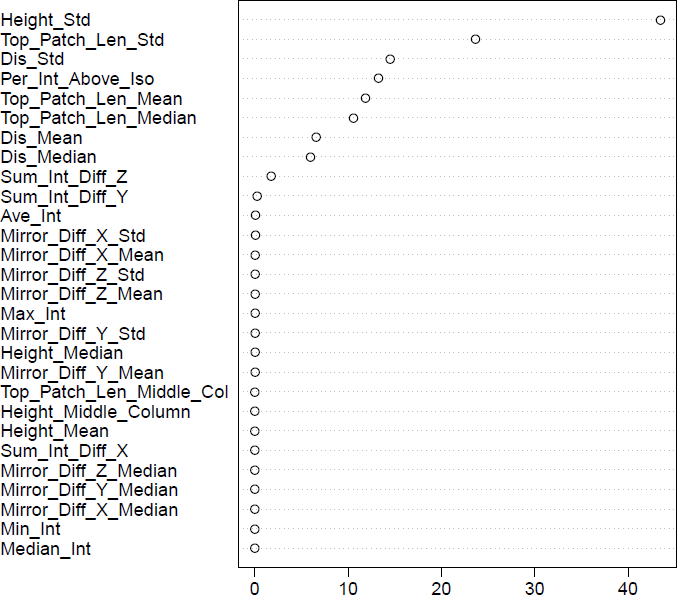
\includegraphics[width=.67\textwidth]{img/dead/c0_random_forest}
				\caption{Importance of variables, identified using Random Forest.}
				\label{fig:c0_RandomForest}
		\end{figure}
		

	
	
	
\subsection{{\color{red} **New : }Probabilistic Field derived from Weighted K-Nearest Neighbours Algorithm }


\par Once the ten most significant variables are identified using the Random Forest, the $k-$nearest neighbour algorithm is applied to generate a probabilistic field. As mentioned in Section \ref{sec:3DpriorsGeneration}, from DASOS we export training feature vectors of dead and alive trees. There are positive training feature vectors from dead trees and negative feature vectors for alive trees. To reduce bias, the number of dead and alive trees used are the same for each test case. 

\par Let’s assume that  $T$ is a training dataset with $n$ feature vectors:
\begin{eqnarray}
T  : \big(x_n, f(x_n) \big), n=1\dots N. 
\end{eqnarray}

The outputs of function $f(x_n) \in \{\textrm{0, 1} \}$. The value $0$ indicates that the feature vector $x_n$ was derived from an alive tree and the value $1$ from a dead tree. For example the dataset $T$ has this form:
\begin{eqnarray}
T : (\boldsymbol{t_1}, 1), (\boldsymbol{t_2}, 0), (\boldsymbol{t_3}, 0), (\boldsymbol{t_4}, 1) . ...... (\boldsymbol{t_n}, 1)
\end{eqnarray}

\par Every feature vector  $\boldsymbol{t_q} \in T$ contains the $10$ most important features exported from DASOS, as they were identified from the Random Forest algorithm ($\boldsymbol{t}=\{t_1, t_2, \dots , t_{10}\}$). Additionally, every feature is associated with a weight value according to its importance ($\boldsymbol{w}=\{w_1,w_2, \dots ,w_{10} \} $). Additionally:


\begin{gather*}
\begin{align}
\boldsymbol{t_q} 
\begin{cases}
t_1\\    
t_2\\
\dots \\
t_{10} \\ 
\end{cases}
\in R^d &  & \boldsymbol{w}
\begin{cases}
w_1\\    
w_2\\
\dots \\
w_{10} \\    
\end{cases}
\in R^d 
\end{align}
\end{gather*}


\par Let's define a data vector $\boldsymbol{x}=(x_1,\dots,x_10)$ of an unknown population. How do we calculate the probability of vector $\boldsymbol{x}$ to belong to the dead trees population? At first, the weighted Euclidean distance from $\boldsymbol{x}$ to every $\boldsymbol{t_q} \in T$ is calculated as follow:
\begin{equation} 
d(\boldsymbol{t_q},\boldsymbol{x}) = \sqrt{\sum_{i=1}^{10}{ \Big(w_i \times (t_{qi}-x_i)^2 \Big)}}
\end{equation}


\par Then the $k-$nearest training samples are selected. In this project $k=7$ was considered reasonable in respect to the size of each testing case. In the future, testing different values of $k$ could evaluate how well the algorithm performs in relation to $k$. The nearest $7$ indices of the training samples are selected as follow:
\begin{equation} 
q = \operatornamewithlimits{argmin}_{\boldsymbol{t} \in T} d(\boldsymbol{t},\boldsymbol{x})
\end{equation}
\par The dataset $V=\{\boldsymbol{v_1}, \boldsymbol{v_2},\dots, \boldsymbol{v_7}\} $ is a subset of the training samples $T$ and contains the k-nearest indices to $\boldsymbol{x}$. The dataset $V$ may contains samples derived from either dead trees, alive trees or both. 


\par For each $\boldsymbol{v_i} \in V$ a weight $\boldsymbol{u_i}$ is calculated:
\begin{equation} 
u_i = \frac{1}{d(\boldsymbol{t_i}, \boldsymbol{i})}
\end{equation}

\par By the end, the probability of a dead tree is given by the following equation: 

\begin{equation} 
P(\textrm{dead}) =  \frac{\sum_{i=1}^{k}{ \Big(u_i \times \delta \big(1,f(\boldsymbol{v_i})\big)\Big)}}{ \sum_{i=1}^{k}{\Big(u_i \times \delta \big(1,f(\boldsymbol{v_i})\big)\Big)} + \sum_{i=1}^{k}{ \Big(u_i \times \delta \big(0,f(\boldsymbol{v_i})\big)\Big)}}
\end{equation}

where the function $\delta(a,b)$ returns $1$ if $a$ is equal to $b$ and $0$ otherwise. 

\par For each column of the voxelised FW LiDAR data, a testing data vector $\boldsymbol{x}$ is created and its probability of been dead is calculated. Figure \ref{fig:c1_knn} shows the probability field the dead trees population. The big circle is the location of the fieldplot and the small circles are the locations of the dead trees. Please note that the white spots contain no data. Those spots appear either when no LiDAR pulse passes through a column or when the pre-defined height of the shape used to calculate the corresponding feature vector is bigger than the elevation of this point. 

 				\begin{figure} [h!]			
 					\centering
 					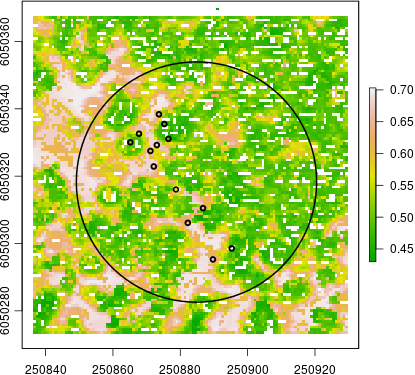
\includegraphics[width=.49\textwidth]{img/dead/c1_knn}
 					\caption{The results of the K-NN algorithm} 
 					\label{fig:c1_knn}
 				\end{figure}

 
 
  \subsection{Filtering}\label{sec:filtering}
  As shown in Figure Figure \ref{fig:c1_knn}, there is Salt and Pepper noise. This noise is removed using a median filter which assigns to every empty pixel the median value of its non-empty neighbouring pixels  (Figure \ref{fig:c2_SaltPepper}). A smoothing filter is further applying for further noise reduction (Figure \ref{fig:c3_Smoothed}). 

	 \begin{figure} [h!]				   
	   \begin{subfigure}[t]{.49\textwidth}
	   \centering
	   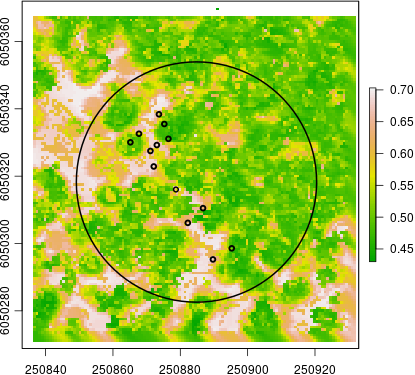
\includegraphics[width=\textwidth]{img/dead/c2_knn_SaltPepper}
	   \caption{`Salt and Pepper' noise reduction} 
	   \label{fig:c2_SaltPepper}
	   \end{subfigure}
	   \begin{subfigure}[t]{.49\textwidth}
	   \centering
	   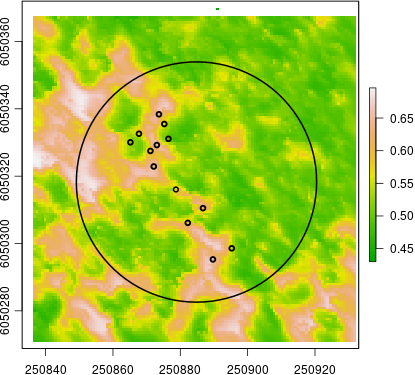
\includegraphics[width=\textwidth]{img/dead/c3_knn_smoothed}
	   \caption{Filtering using a smoothing kernel} 
	   \label{fig:c3_Smoothed}
	   \end{subfigure}
	   \caption{Filtering the results of te K-NN algorithm}  
	   \label{fig:salt_smooth} 
	\end{figure}

 \newpage
 \subsection{Removing Ground Pixels}\label{sec:groundMask}
 \par Removing the ground pixels is a trivial task because the DTM has already subtracted from the data and therefore the height of the ground is approximately constant. A histogram of the height values was generated. As shown in Figure \ref{fig:c5_heightHist}, there are three well-defined classes (ground, trees and noise). The ground and noise are removed using two thresholds. This processed is illustrated in Figure \ref{fig:GroundPixelsRemoval}.

 \begin{figure} [h!]			
 	\begin{subfigure}[t]{.49\textwidth}
 		
 		\centering
 		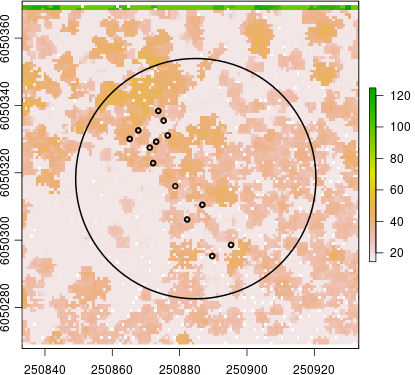
\includegraphics[width=\textwidth]{img/dead/c4_height}
 		\caption{DEM of plot}
 		\label{fig:c4_height}
 	\end{subfigure} \hfill
 	\begin{subfigure}[t]{.49\textwidth}
 		\centering
 		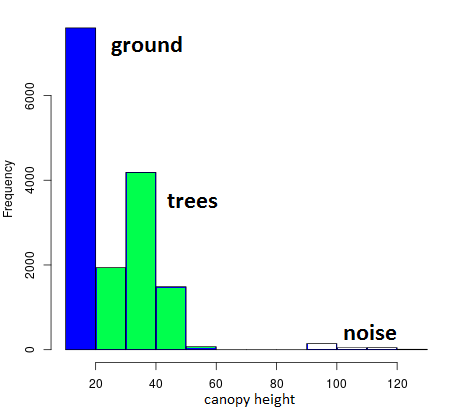
\includegraphics[width=\textwidth]{img/dead/c5_histHeight}
 		\caption{Histogram of heights} 
 		\label{fig:c5_heightHist}
 	\end{subfigure} \hfill
 	\begin{subfigure}[t]{.49\textwidth}
 		\centering
 		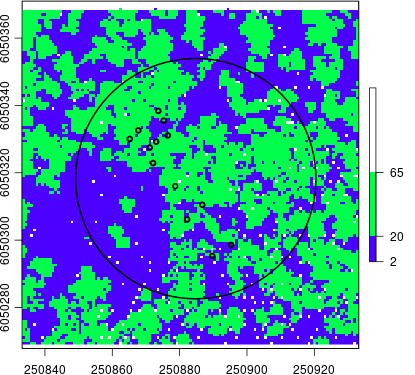
\includegraphics[width=\textwidth]{img/dead/c6_groundThres}
 		\caption{Thresholds} 
 		\label{fig:c6_groundMask}
 	\end{subfigure}
 	\begin{subfigure}[t]{.49\textwidth}
 		\centering
 		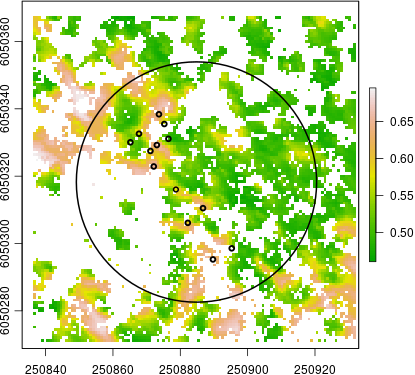
\includegraphics[width=\textwidth]{img/dead/c7_groundRemoved}
 		\caption{Results} 
 		\label{fig:c7_groundRemoved}
 	\end{subfigure}
 	\caption{Removing the ground pixels}  
 	\label{fig:GroundPixelsRemoval} 
 \end{figure}
 
 


 \subsection{Dead and Alive Threshold, Filtering, Segmentation and Position Assignment }\label{sec:Segmentation}

  \par In order to obtain the estimated positions of the dead trees, there are four steps left:
  \begin{enumerate}
  	\item Thresholding 
  	\item Filtering
  	\item Segmentation
  	\item Position assignment 
  \end{enumerate}
  
  \par Up to this stage, we have an image of the probabilistic field and the ground has been removed (Figure \ref{fig:c7_groundRemoved}). After that a threshold for separating dead and alive pixels is chosen using the training data and the alive pixels are removed (Figure \ref{fig:c8_deadThres}). The output image contains out-liners; pixels which are classified as dead but have no neigbouring pixels classified as dead. To reduce over-detection of dead trees, these pixels are filtered out (Figure \ref{fig:c9_sharpFilter}). Afterwards, the pixels are grouped into trees relatively to their neighbouring pixels using a seed growth segmentation algorithm (Algorithm \ref{alg:seedGrownth} and Figure \ref{fig:c10_segmentation}). By the end, it is assumed that each segment $S$ is a dead tree and its position is calculated by taking the average geo-spatial location of the pixels that belong in segment $S$ (Figure \ref{fig:c11_results}). 
 
 

  \begin{figure} [h!]			
  	\begin{subfigure}[t]{.49\textwidth}
  		
  		\centering
  		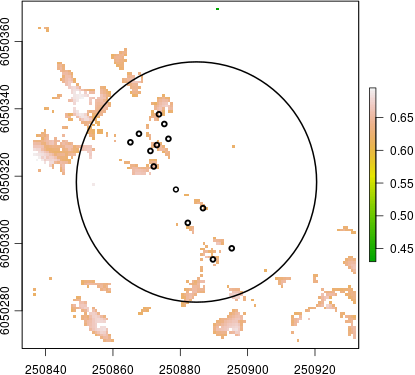
\includegraphics[width=\textwidth]{img/dead/c8_thresDead}
  		\caption{Thresholding dead from alive trees}
  		\label{fig:c8_deadThres}
  	\end{subfigure} \hfill
  	\begin{subfigure}[t]{.49\textwidth}
  		\centering
  		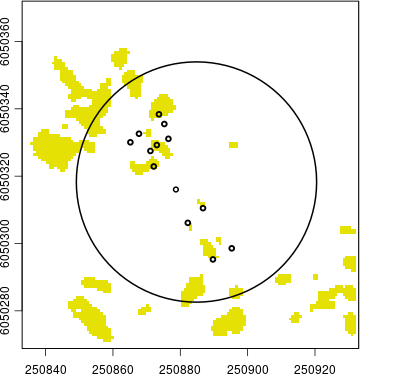
\includegraphics[width=\textwidth]{img/dead/c9_sharpFilter}
  		\caption{Noise Reduction} 
  		\label{fig:c9_sharpFilter}
  	\end{subfigure} \hfill
  \caption{Thresholding and filtering }  
  \label{fig:dt_sf} 
  \end{figure}
  
  \begin{figure} [h!]			
  	\begin{subfigure}[t]{.49\textwidth}
  		\centering
  		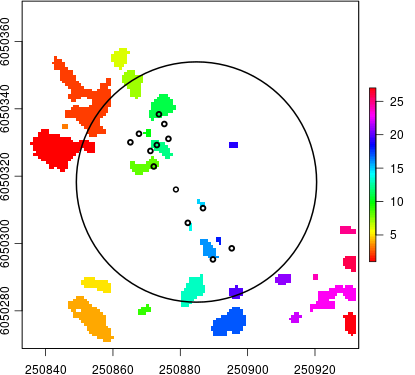
\includegraphics[width=\textwidth]{img/dead/c10_segmentationResults}
  		\caption{Segmentation using a seed grownth algortihm}
  		\label{fig:c10_segmentation}
  	\end{subfigure}
  	\begin{subfigure}[t]{.49\textwidth}
  		\centering
  		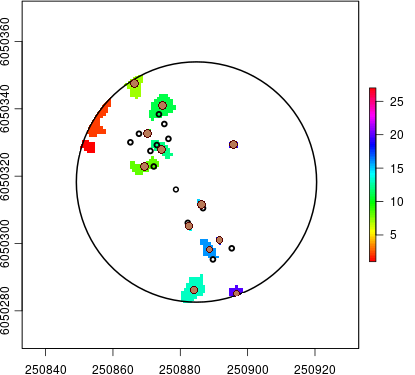
\includegraphics[width=\textwidth]{img/dead/c11_TreePos}
  		\caption{The estimated dead tree positions (brown dots)} 
  		\label{fig:c11_results}
  	\end{subfigure}
  	\caption{Segmentation and calculating the dead trees' position. }  
  	\label{fig:segm_results} 
  \end{figure}
  

 \begin{algorithm}
 	\caption{Seed growth algorithm for segmenting pixels classified as dead}
 	\label{alg:seedGrownth}
 	\centering
 	\begin{algorithmic}[1]
 		\State $P \gets $ all pixels classified as dead  %\boldsymbol{
 		\State $s \gets $ 0 
 		\While { not reached the end of set P}
        \State get next pixel $\boldsymbol{p} \in P$ that is not assigned to a segment
 		\State  Assign pixel $\boldsymbol{p} $ to segment $s$
 		\State  find $K(\boldsymbol{p_1},\dots, \boldsymbol{p_n})$ such that $K \subseteq P$ and every $\boldsymbol{p_i} \in K$ is a neighbour of $\boldsymbol{p}$
 		\State $ \forall \space \boldsymbol{p_i} \in K $, $\boldsymbol{p} \gets \boldsymbol{p_i}$ and repeat from line 5
 		\State all pixels of segment $s$ has been labelled
 		\State $s \gets s + 1 $
 		\EndWhile
 	\end{algorithmic}
 \end{algorithm}



\section{Evaluation} 
\par The results are evaluated into two different ways: 
\begin{itemize}
	\item Firstly, the predicted locations of the dead trees are evaluated in relation to their distance from the actual dead trees. Example of output is given in Figure \ref{fig:c11_results}. 
	\item Secondly, a pixelwise evaluation is done using the image produced with the prediction of whether a column from the voxelised FW LiDAR contains information from a dead tree or not. Example of output result is given in Figure \ref{fig:c9_sharpFilter}.	
\end{itemize}

\par Both results have been cross-validated using the fieldplots division depicted in Figure \ref{fig:DASOSsPriors}. The 50 field plots are divided into 5 datasets and each dataset uses 10 plots for testing and the rest 40 for evaluation. Additionally, an extra dataset that uses 30 plots for training and 20 for evaluation was created to check whether the increase amount of training samples improves the precision and recall of the results. For each dataset, feature vectors of processed and raw intensities are generated. But Random Forest failed to identify important variable from the feature vectors with the raw intensities due to the irregular shapes of the dead trees. For that reason, results were only obtained from processed voxel intensity values. The feature vectors with raw intensities should be used in other application where trees/object shapes are similar. Additionally, for the second evaluation a random set of results was generated for comparison. This random prediction uses the probability of a squared meter to contain a dead tree or not and the number of dead trees assigned to it is approximately the same as the number of dead trees that exist within the field data.



   \subsection{Distance Related Evaluation}
   
   
\begin{table}[!htbp]
	% increase table row spacing, adjust to taste
	\renewcommand{\arraystretch}{1.3}
	% if using array.sty, it might be a good idea to tweak the value of
	% \extrarowheight as needed to properly center the text within the cells
	
	\centering
	% Some packages, such as MDW tools, offer better commands for making tables
	% than the plain LaTeX2e tabular which is used here.
	\begin{tabular}{|P{2.1cm}|P{0.75cm}|P{0.75cm}|P{0.75cm}|P{0.75cm}|P{0.75cm}|P{0.75cm}|P{0.75cm}|P{0.75cm}|P{0.75cm}|P{0.75cm}|}
		\hline
		
		\multicolumn{11}{|c|}{ \textbf{Precision (\%)}}	\\ \hline
		Distance (m)	&	1	&	2	&	3	&	4	&	5	&	6	&	7	&	8	&	9	&	10	\\ \hline
D1	&	7.29	&	12.15	&	16.1	&	24.31	&	32.21	&	38.9	&	47.11	&	49.84	&	56.23	&	58.35	\\ \hline
D2	&	2	&	3.67	&	8.36	&	18.39	&	25.08	&	33.11	&	35.78	&	40.13	&	46.48	&	50.5	\\ \hline
D3	&	1.48	&	5.46	&	14.2	&	23.32	&	29.08	&	36.6	&	40.23	&	46.15	&	51.38	&	56.28	\\ \hline
D4	&	0.96	&	7.24	&	20.04	&	28.26	&	33.09	&	40.09	&	44.68	&	52.17	&	56.28	&	62.07	\\ \hline
D5	&	0.75	&	5.26	&	8.27	&	12.03	&	14.28	&	21.8	&	28.57	&	39.84	&	47.36	&	55.63	\\ \hline
D\_1\_2\_3	&	0	&	8.69	&	13.04	&	19.13	&	24.34	&	29.56	&	34.78	&	36.52	&	41.73	&	55.65	\\ \hline
\hline \hline
\multicolumn{11}{|c|}{ 	\textbf{Recall (\%)}} \\ \hline
Distance (m)	&	2.55	&	9.26	&	18.84	&	32.26	&	45.04	&	53.35	&	56.23	&	58.78	&	63.25	&	68.05	\\ \hline
D1	&	8.22	&	13.48	&	23.02	&	31.25	&	38.48	&	51.31	&	62.17	&	65.78	&	66.11	&	69.07	\\ \hline
D2	&	6.69	&	14.49	&	26.55	&	34.77	&	40.97	&	48.6	&	56.61	&	59.18	&	60.71	&	63.41	\\ \hline
D3	&	5.16	&	15.5	&	30.09	&	38.29	&	43.46	&	45.89	&	51.06	&	52.58	&	55.31	&	57.75	\\ \hline
D4	&	0.89	&	4.45	&	12.75	&	24.03	&	29.37	&	35.9	&	41.83	&	49.85	&	59.34	&	61.12	\\ \hline
D5	&	0	&	7.22	&	14.45	&	20.07	&	45.19	&	50.6	&	51.8	&	62.65	&	63.85	&	73.49	\\ \hline
D\_1\_2\_3	&	0	&	0	&	6.17	&	7.33	&	8.88	&	10.03	&	12.74	&	20.84	&	21.62	&	33.59	\\ \hline
	\end{tabular}
	\caption{Distance based evaluation: This table gives the percentage of precision and recall achieved using the cylindrical shape to extract features.}
	\label{tab:CylinderResults}
\end{table}


   \begin{figure} [h!]
   	\centering
   	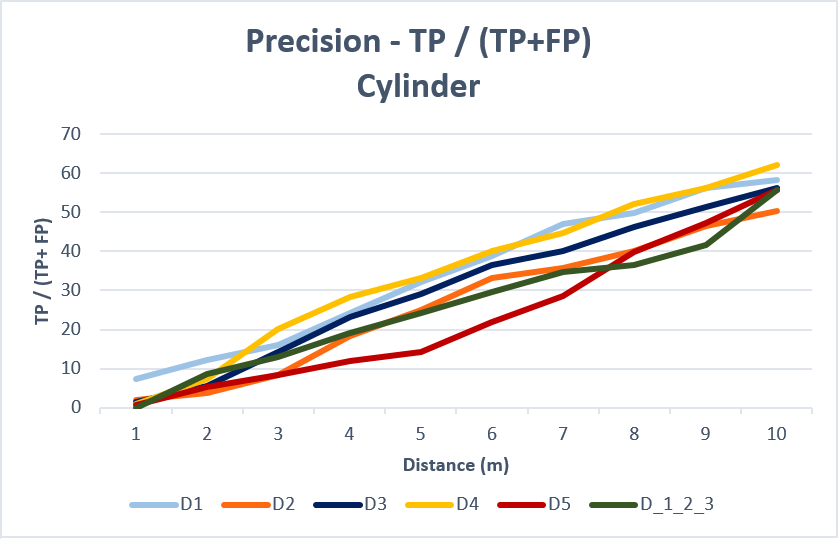
\includegraphics[width=\textwidth]{img/dead/results/Precision_Cylinder}
   	\caption{}
   	\label{fig:Precision_Cylinder}
   \end{figure}
   
     \begin{figure} [h!]
     	\centering
     	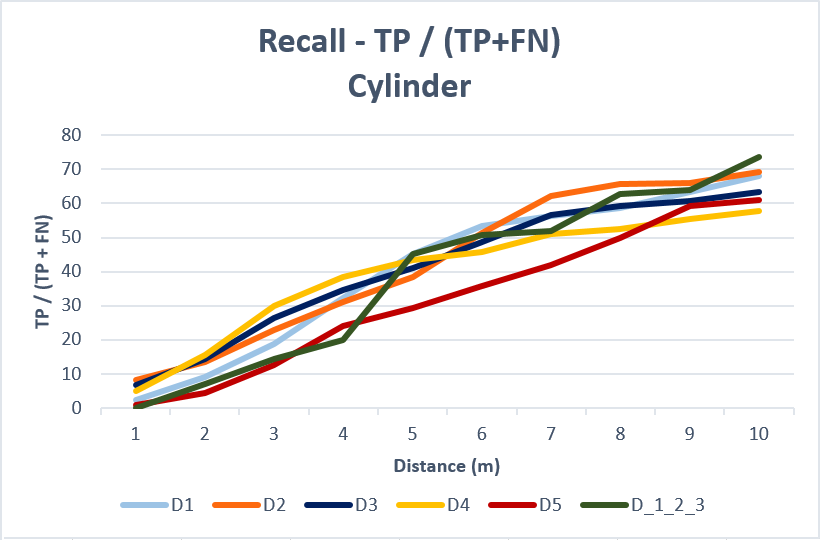
\includegraphics[width=\textwidth]{img/dead/results/Recall_Cylinder}
     	\caption{}
     	\label{fig:Recall_Cylinder}
     \end{figure}
     
     
\begin{table}[!htbp]
	% increase table row spacing, adjust to taste
	\renewcommand{\arraystretch}{1.3}
	% if using array.sty, it might be a good idea to tweak the value of
	% \extrarowheight as needed to properly center the text within the cells
	
	\centering
	% Some packages, such as MDW tools, offer better commands for making tables
	% than the plain LaTeX2e tabular which is used here.
	\begin{tabular}{|P{2.1cm}|P{0.75cm}|P{0.75cm}|P{0.75cm}|P{0.75cm}|P{0.75cm}|P{0.75cm}|P{0.75cm}|P{0.75cm}|P{0.75cm}|P{0.75cm}|}
		\hline
		
		\multicolumn{11}{|c|}{ \textbf{Precision (\%)}}	\\ \hline
Distance (m)	&	1	&	2	&	3	&	4	&	5	&	6	&	7	&	8	&	9	&	10	\\ \hline
D1	&	7.78	&	10.47	&	14.07	&	24.85	&	32.63	&	40.11	&	47.9	&	53.59	&	59.28	&	61.97	\\ \hline
D2	&	3.66	&	12.5	&	16.37	&	22.84	&	26.72	&	34.26	&	42.02	&	46.76	&	51.72	&	56.68	\\ \hline
D3	&	1.24	&	3.42	&	20.56	&	25.23	&	29.28	&	36.76	&	41.74	&	43.92	&	50.15	&	53.27	\\ \hline
D4	&	8.36	&	19.86	&	33.79	&	36.58	&	39.02	&	44.25	&	50.52	&	55.05	&	63.76	&	66.89	\\ \hline
D5	&	1.96	&	1.96	&	5.88	&	15.68	&	19.6	&	25.49	&	35.29	&	41.17	&	45.09	&	62.74	\\ \hline
\hline \hline
\multicolumn{11}{|c|}{ 	\textbf{Recall (\%)}} \\ \hline
Distance (m)	&	1	&	2	&	3	&	4	&	5	&	6	&	7	&	8	&	9	&	10	\\ \hline
D1	&	9.58	&	19.16	&	35.14	&	44.4	&	50.47	&	56.86	&	62.93	&	65.49	&	69.96	&	74.76	\\ \hline
D2	&	10.52	&	20.39	&	33.22	&	37.82	&	47.36	&	62.17	&	67.1	&	70.39	&	74.01	&	75.65	\\ \hline
D3	&	5.48	&	20	&	31.93	&	38.7	&	46.12	&	54.83	&	60.64	&	67.09	&	72.9	&	77.09	\\ \hline
D4	&	7.9	&	17.93	&	24.92	&	26.74	&	33.13	&	38.29	&	45.28	&	47.41	&	50.75	&	52.27	\\ \hline
D5	&	4.74	&	4.74	&	5.34	&	11.86	&	16.02	&	16.32	&	21.95	&	23.73	&	27.29	&	31.75	\\ \hline
	\end{tabular}
	\caption{Distance based evaluation: This table gives the percentage of precision and recall achieved using the Cuboid shape to extract features.}
	\label{tab:CuboidResults}
\end{table}

        \begin{figure} [h!]
        	\centering
        	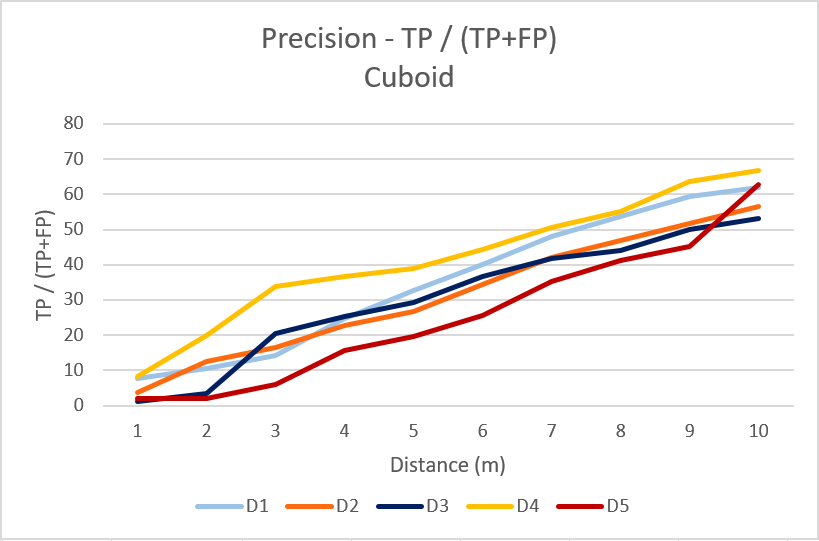
\includegraphics[width=\textwidth]{img/dead/results/Precision_Cuboid}
        	\caption{}
        	\label{fig:Precision_Cuboid}
        \end{figure}
    
        \begin{figure} [h!]
        	\centering
        	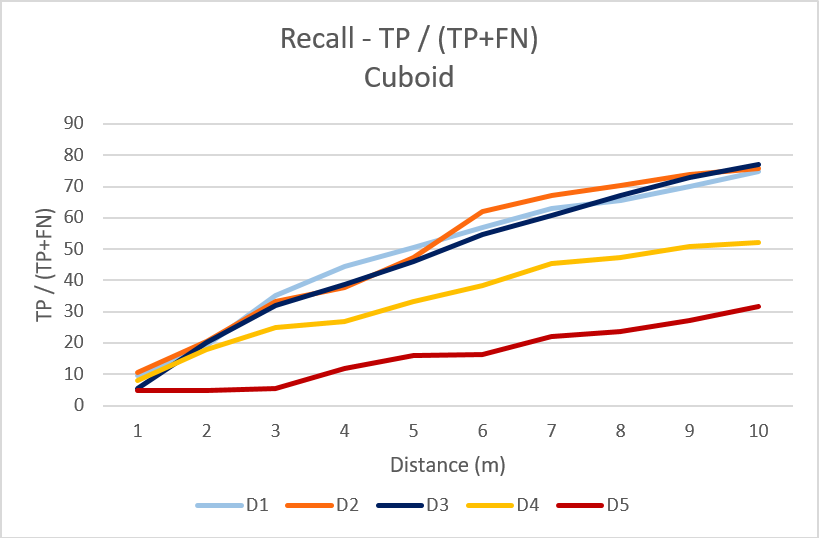
\includegraphics[width=\textwidth]{img/dead/results/Recall_Cuboid}
        	\caption{}
        	\label{fig:Recall_Cuboid}
        \end{figure}
    
        
\begin{table}[!htbp]
	% increase table row spacing, adjust to taste
	\renewcommand{\arraystretch}{1.3}
	% if using array.sty, it might be a good idea to tweak the value of
	% \extrarowheight as needed to properly center the text within the cells
	
	\centering
	% Some packages, such as MDW tools, offer better commands for making tables
	% than the plain LaTeX2e tabular which is used here.
	\begin{tabular}{|P{2.1cm}|P{0.75cm}|P{0.75cm}|P{0.75cm}|P{0.75cm}|P{0.75cm}|P{0.75cm}|P{0.75cm}|P{0.75cm}|P{0.75cm}|P{0.75cm}|}
		\hline
		
		\multicolumn{11}{|c|}{ \textbf{Precision (\%)}}		\\ \hline
		Distance (m)&	1	&	2	&	3	&	4	&	5	&	6	&	7	&	8	&	9	&	10	\\ \hline
		Cylinder	&	2.50	&	6.76	&	13.40	&	21.27	&	26.75	&	34.10	&	39.28	&	45.63	&	51.55	&	56.57	\\ \hline
		Cuboid	&	4.60	&	9.645	&	18.14	&	25.04	&	29.45	&	36.18	&	43.50	&	48.10	&	54.00	&	60.31	\\ \hline
		Random	&	0	&	0	&	2.56	&	8.06	&	11.36	&	23.81	&	52.75	&	57.14	&	72.16	&	79.49	\\ \hline
		Cylinder 1\_2\_3	&	0	&	8.696	&	13.04	&	19.13	&	24.35	&	29.57	&	34.78	&	36.52	&	41.74	&	55.65	\\ \hline
		\hline \hline
		\multicolumn{11}{|c|}{ 	\textbf{Recall (\%)}} \\ \hline
		Distance (m)&	1	&	2	&	3	&	4	&	5	&	6	&	7	&	8	&	9	&	10	\\ \hline
		Cylinder	&	4.71	&	11.44	&	22.26	&	32.13	&	39.47	&	47.02	&	53.58	&	57.24	&	60.95	&	63.88	\\ \hline
		Cuboid	&	7.65	&	16.45	&	26.11	&	31.91	&	38.63	&	45.70	&	51.59	&	54.83	&	59.00	&	62.31	\\ \hline
		Random	&	0	&	0	&	6.18	&	7.34	&	8.88	&	10.04	&	12.74	&	20.85	&	21.62	&	28.59	\\ \hline
		Cylinder 1\_2\_3	&	0	&	7.23	&	14.46	&	20.07	&	45.19	&	50.60	&	51.81	&	62.65	&	63.86	&	73.49	\\ \hline
		
	\end{tabular}
	\caption{Distance based evaluation. This table gives the percentage of precision and recall of the average results of each shape (Cylinder and Cuboid), the Random prediction generated for comparison and the the dataset with that its training dataset is three times larger.}
	\label{tab:AveRanResults}
\end{table}

           \begin{figure} [h!]
           	\centering
           	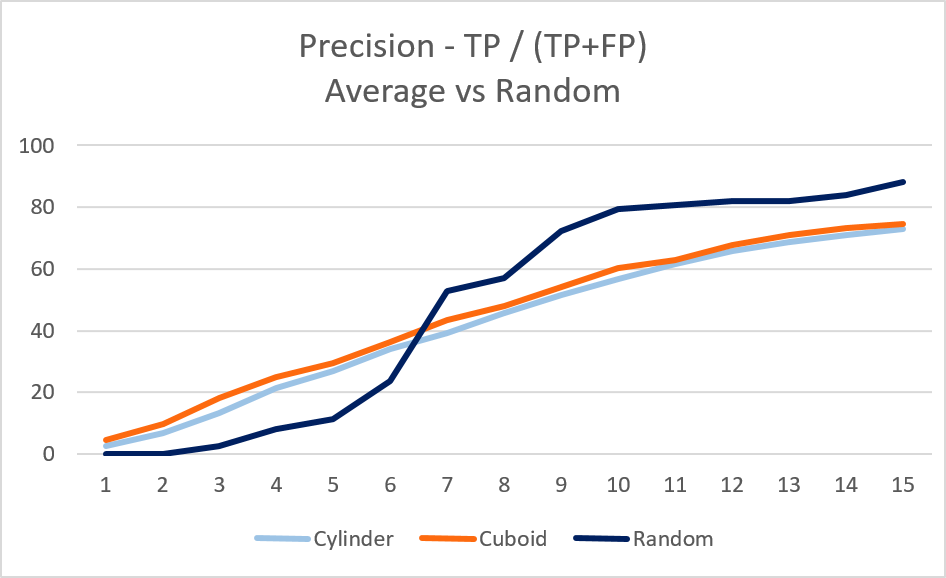
\includegraphics[width=\textwidth]{img/dead/results/Precision_AveRan}
           	\caption{}
           	\label{fig:Precision_AveRan}
           \end{figure}
        
           
           \begin{figure} [h!]
           	\centering
           	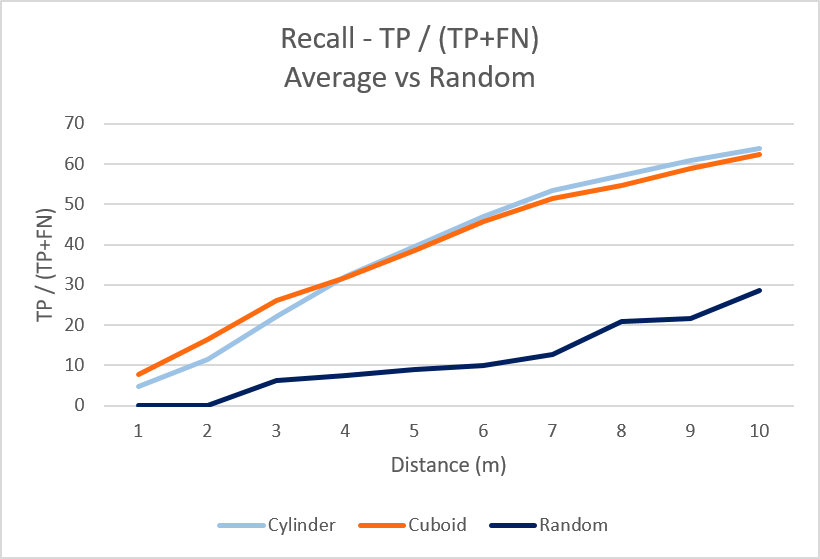
\includegraphics[width=\textwidth]{img/dead/results/Recall_AveRan}
           	\caption{}
           	\label{fig:Recall_AveRan}
           \end{figure}
           
\subsection{Pixelwise Evaluation}

\begin{figure} [h!]
	\centering
	
\includegraphics[width=0.49\textwidth]{img/dead/results/PixewiseEvaluationPlot}
	\caption{Example of plot created for the pixelwise evaluation. The grey pixels indicate areas with dead trees, black is non dead trees and white is either outside the plot or the evaluation blank area because the size of the dead trees is unknown.}
	\label{fig:Pixelwise_evaluation_plot}
\end{figure}


		
\section{Discussion}

\par Dead tree detection is a difficult task due to the irregular shapes of the trees and different sizes. Here we produced this algorithm (pla pla) which is new because it doesn't need tree segmentation but has a lot of room for improvement. 

Also don't know the accuracy of the tree position and as we can see at some heigh maps there are places where there are trees according to the fieldplots but the data clearly shown that there are not trees



\par Here it is worth mentioning that the dead tree detection is the first application of DASOS's 3D priors. 

\section{Future Work}

\begin{itemize}
	\item Manually check and improve position of dead trees using visualisations of the data. In order to improve accuracy of test and evaluating data
	\item Separate trees from field data according to their height because tree with different heights have different shape properties and the priors used had constant size
	\item Create priors that have adjustable size according to the height of the tree	
	\item After the seed growth algorithm, check the size of the segments and look into the possibility of merging two segments into one or dividing a segments into multiple sub-segments.
	\item Test the results when only using dead trees for training data and not alive
	\item The system is usually confused at the edges of the alive trees. Research on how this could be improved. 
\end{itemize}


\end{document}